\documentclass[aspectratio=169,professionalfonts]{beamer}

\usepackage{fontspec}
\usepackage{xeCJK}
\usepackage{booktabs}
\usepackage{array}
\usepackage{tabularx}
\usepackage{hyperref}

\graphicspath{{docs/presentations/images/}{images/}}

\setsansfont{TeX Gyre Heros}
\setmainfont{TeX Gyre Heros}
\setmonofont{DejaVu Sans Mono}
\setCJKmainfont[AutoFakeBold=2]{AR PL UMing CN}
\setCJKsansfont[AutoFakeBold=2]{Droid Sans Fallback}
\setCJKmonofont{Droid Sans Fallback}

\definecolor{criewInk}{HTML}{11202A}
\definecolor{criewCharcoal}{HTML}{24313A}
\definecolor{criewCream}{HTML}{F7F4ED}
\definecolor{criewSand}{HTML}{EDE6D6}
\definecolor{criewOrange}{HTML}{C65D2E}
\definecolor{criewOrangeLight}{HTML}{F3D8CD}
\definecolor{criewTeal}{HTML}{2A7F98}
\definecolor{criewTealLight}{HTML}{DCEFF4}
\definecolor{criewOlive}{HTML}{617A55}
\definecolor{criewOliveLight}{HTML}{E2E8DB}
\definecolor{criewGold}{HTML}{D49B32}
\definecolor{criewGoldLight}{HTML}{F5E8C5}
\definecolor{criewDanger}{HTML}{A74632}
\definecolor{criewDangerLight}{HTML}{F7E1DD}
\definecolor{criewSlate}{HTML}{5F6B73}

\setbeamercolor{normal text}{fg=criewInk,bg=criewCream}
\setbeamercolor{structure}{fg=criewOrange}
\setbeamercolor{frametitle}{fg=criewInk,bg=criewCream}
\setbeamercolor{title}{fg=criewCream,bg=criewInk}
\setbeamercolor{subtitle}{fg=criewGoldLight,bg=criewInk}
\setbeamercolor{block title}{fg=criewInk,bg=criewGoldLight}
\setbeamercolor{block body}{fg=criewInk,bg=criewCream}
\setbeamercolor{block title alerted}{fg=criewDanger,bg=criewDangerLight}
\setbeamercolor{block body alerted}{fg=criewInk,bg=criewCream}
\setbeamercolor{block title example}{fg=criewTeal,bg=criewTealLight}
\setbeamercolor{block body example}{fg=criewInk,bg=criewCream}

\setbeamertemplate{navigation symbols}{}
\setbeamertemplate{footline}{
  \leavevmode
  \hbox{
    \begin{beamercolorbox}[wd=.83\paperwidth,ht=2.8ex,dp=1.2ex,leftskip=1em]{author in head/foot}
      \color{criewSlate}\tiny CRIEW / kernel patch mail workflow
    \end{beamercolorbox}
    \begin{beamercolorbox}[wd=.17\paperwidth,ht=2.8ex,dp=1.2ex,rightskip=1em]{date in head/foot}
      \color{criewSlate}\tiny\insertframenumber/\inserttotalframenumber
    \end{beamercolorbox}
  }
}
\setbeamertemplate{itemize item}{\color{criewOrange}$\blacktriangleright$}
\setbeamertemplate{itemize subitem}{\color{criewTeal}$\bullet$}

\newcommand{\sectiontitle}[1]{
  \begin{beamercolorbox}[wd=\linewidth,sep=0.7em,rounded=true]{block title}
    \usebeamerfont*{frametitle}\Large\bfseries #1
  \end{beamercolorbox}
  \vspace{0.4em}
}

\newcommand{\statcard}[3]{
  \begin{beamercolorbox}[wd=\linewidth,sep=0.8em,rounded=true]{#1}
    {\bfseries #2}\par
    \vspace{0.3em}
    #3
  \end{beamercolorbox}
}

\title{从内核开发流程到邮件协作}
\subtitle{用 CRIEW 更轻松上手 Linux kernel 邮件工作流}
\author{CRIEW 项目介绍}
\date{2026-04-10}

\begin{document}

\begin{frame}[plain]
  \setbeamercolor{background canvas}{bg=criewInk}
  \vspace{0.3cm}
  {\color{criewGold}\Large\bfseries CRIEW 项目介绍}\par
  \vspace{0.5cm}
  {\color{criewCream}\fontsize{24}{28}\selectfont\bfseries 从内核开发流程到邮件协作}\par
  \vspace{0.35cm}
  {\color{criewGoldLight}\large 用 CRIEW 更轻松上手 Linux kernel 邮件工作流}\par
  \vspace{0.55cm}
  {\color{criewCream}\normalsize 订阅 $\rightarrow$ 同步 $\rightarrow$ 阅读 $\rightarrow$ 应用 patch $\rightarrow$ 回信}\par
  \vspace{0.8cm}
  \begin{columns}[T,totalwidth=\textwidth]
    \begin{column}{0.58\textwidth}
      \begin{beamercolorbox}[wd=\linewidth,sep=1em,rounded=true]{block body example}
        \color{criewInk}
        \textbf{这份分享的目标}\par
        \vspace{0.35em}
        先讲 Linux kernel 的邮件式开发流程，再讲 CRIEW 如何把这条流程变成新人也能持续使用的终端工作流。
      \end{beamercolorbox}
      \vspace{0.45cm}
      {\color{criewCream}\small Terminal-first / Local-first / Mail-native}
    \end{column}
    \begin{column}{0.38\textwidth}
      \begin{beamercolorbox}[wd=\linewidth,sep=1em,rounded=true]{block body}
        \color{criewInk}
        \textbf{一句话定位}\par
        \vspace{0.35em}
        CRIEW 不是另一个 GUI 邮件客户端，而是面向 kernel patch 邮件协作的 Rust TUI 工作台。
      \end{beamercolorbox}
    \end{column}
  \end{columns}
\end{frame}

\begin{frame}
  \sectiontitle{这场交流会会怎么进行}
  \scriptsize
  \begin{columns}[T,totalwidth=\textwidth]
    \begin{column}{0.48\textwidth}
      \statcard{block body example}{1 先讲传统流程}{
        先用 Linux kernel 的邮件式开发流程建立共同上下文，看 mailing list、patch series 和 reroll 为什么会这样运作。
      }
      \vspace{0.35em}
      \statcard{block body}{2 再拆 patch 与 thread}{
        接着看一封 PATCH 文件长什么样，以及 review reply、v2 / v3 在邮件 thread 里怎么串起来。
      }
    \end{column}
    \begin{column}{0.48\textwidth}
      \statcard{block body alerted}{3 然后看 CRIEW demo}{
        再切到 CRIEW，看看它如何把 thread 阅读、patch apply 和 reply 组织进同一个 TUI 工作流。
      }
      \vspace{0.35em}
      \statcard{block body}{4 最后讲现状与参与}{
        最后会讲项目目前到了什么阶段、适合谁现在试，以及会后怎么安装、反馈和参与贡献。
      }
    \end{column}
  \end{columns}
  \vspace{0.35em}
  \begin{beamercolorbox}[wd=\linewidth,sep=0.65em,rounded=true]{block title}
    \textbf{节奏：}这份内容按 30 到 60 分钟准备；中间适合穿插 live demo，最后留出讨论和问答。
  \end{beamercolorbox}
\end{frame}

\begin{frame}
  \sectiontitle{为什么内核开发仍然以邮件为中心}
  \begin{columns}[T,totalwidth=\textwidth]
    \begin{column}{0.42\textwidth}
      \begin{beamercolorbox}[wd=\linewidth,sep=1em,rounded=true]{block title example}
        \Large\bfseries Linux kernel 的协作单位\\[0.25em]
        不是 PR，\\
        而是 patch series + thread
      \end{beamercolorbox}
      \vspace{0.5em}
      \begin{beamercolorbox}[wd=\linewidth,sep=0.8em,rounded=true]{block body}
        一封 patch 邮件只是开始；真正的协作发生在整个线程里。
      \end{beamercolorbox}
    \end{column}
    \begin{column}{0.54\textwidth}
      \begin{columns}[T,totalwidth=\linewidth]
        \begin{column}{0.48\linewidth}
          \statcard{block body alerted}{公开讨论}{
            改动发到邮件列表，review 对所有人可见。
          }
          \vspace{0.55em}
          \statcard{block body example}{线程上下文}{
            后续意见通过 reply 累积在同一 thread。
          }
        \end{column}
        \begin{column}{0.48\linewidth}
          \statcard{block body}{多轮修订}{
            v2 / v3 / RESEND 是常态，不是例外。
          }
          \vspace{0.55em}
          \statcard{block body}{合入路径}{
            maintainer 从邮件线程收集 trailer，再带入自己的 tree。
          }
        \end{column}
      \end{columns}
    \end{column}
  \end{columns}
\end{frame}

\begin{frame}
  \sectiontitle{网页上的 mailing list 是什么样子}
  \begin{center}
    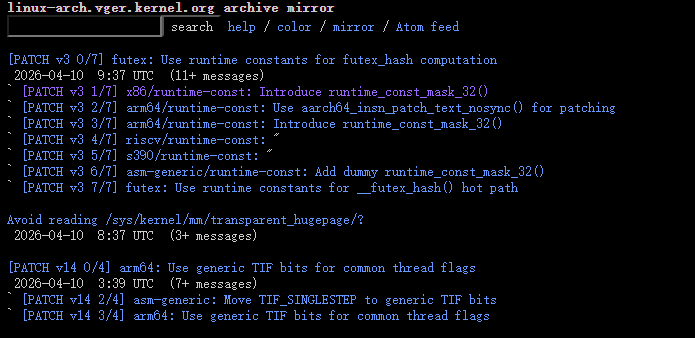
\includegraphics[width=\linewidth,height=0.6\textheight,keepaspectratio]{linux-arch-mailing-list.png}
  \end{center}
  \vspace{0.15em}
  {\scriptsize
    \textbf{示例入口：}\par
    \href{https://subspace.kernel.org/vger.kernel.org.html}{\texttt{https://subspace.kernel.org/vger.kernel.org.html}}\par
    \href{https://lore.kernel.org/linux-arch/}{\texttt{https://lore.kernel.org/linux-arch/}}
  }
\end{frame}

\begin{frame}
  \sectiontitle{一条 patch 从想法到合入，大致会经历什么}
  \small
  \begin{tabularx}{\textwidth}{>{\bfseries}p{0.13\textwidth} >{\raggedright\arraybackslash}X >{\raggedright\arraybackslash}X}
    \toprule
    阶段 & 关键动作 & 典型关注点 \\
    \midrule
    1 选基线 & 找对 subsystem 与 maintainer tree & 你改的东西归谁维护 \\
    2 拆 commits & 一补丁一件事，写清 commit message & patch 粒度能否被 review \\
    3 形成 series & cover letter + [PATCH vN M/N] & 线程是否可持续迭代 \\
    4 本地自检 & checkpatch / 编译 / 功能测试 & 不把低级问题扔给 reviewer \\
    5 选收件人 & get\_maintainer.pl 或 b4 prep --auto-to-cc & To/Cc 列表是否对 \\
    6 发邮件 & git send-email 或 b4 send & 保住邮件线程关系 \\
    7 Reroll & 读 review，回复并修成 v2 / v3 & changelog 和回复质量 \\
    \bottomrule
  \end{tabularx}
  \vspace{0.6em}
  \begin{beamercolorbox}[wd=\linewidth,sep=0.7em,rounded=true]{block body example}
    \textbf{核心点：}关键不是一次 push，而是围绕 thread 的持续讨论与修订。
  \end{beamercolorbox}
\end{frame}

\begin{frame}[fragile]
  \sectiontitle{传统 Linux patch 流程，命令层面大概长这样}
  \scriptsize
  \begin{columns}[T,totalwidth=\textwidth]
    \begin{column}{0.49\textwidth}
      \begin{beamercolorbox}[wd=\linewidth,sep=0.75em,rounded=true]{block body}
{\ttfamily
git clone https://git.kernel.org/.../linux.git\\
cd linux\\
git checkout -b fix-arch-bug\\
\$EDITOR arch/...\\
make -j\$(nproc)\\
git add arch/...\\
git commit -s\\
git format-patch -1
}
      \end{beamercolorbox}
      \vspace{0.45em}
      \begin{beamercolorbox}[wd=\linewidth,sep=0.7em,rounded=true]{block body example}
        第一段链路还只是本地开发：改代码、编译、自测、整理出 patch 文件。
      \end{beamercolorbox}
    \end{column}
    \begin{column}{0.49\textwidth}
      \begin{beamercolorbox}[wd=\linewidth,sep=0.75em,rounded=true]{block body alerted}
{\ttfamily
./scripts/checkpatch.pl 0001-*.patch\\
./scripts/get\_maintainer.pl -f arch/...\\
git send-email 0001-*.patch\\
\# 去 lore 里继续看 thread / 收 review\\
git commit --amend -s\\
git format-patch -v2 -1\\
git send-email 0001-v2-*.patch
}
      \end{beamercolorbox}
      \vspace{0.45em}
      \begin{beamercolorbox}[wd=\linewidth,sep=0.7em,rounded=true]{block title}
        \textbf{难点：}单条命令都不复杂，但收件人、thread、版本号和上下文关系都要自己维护。
      \end{beamercolorbox}
    \end{column}
  \end{columns}
\end{frame}

\begin{frame}[fragile]
  \sectiontitle{一个 PATCH 文件实际长什么样}
  \fontsize{6.5}{7.2}\selectfont
  \begin{columns}[T,totalwidth=\textwidth]
    \begin{column}{0.48\textwidth}
      \begin{exampleblock}{邮件头 + 提交说明}
\begin{semiverbatim}
From abcdef1234567890 Mon Sep 17 00:00:00 2001
From: Alice Dev <a@example.com>
Subject: [PATCH v2 1/1] arch: fix boot order

Fix the fallback order in early boot path.

Signed-off-by: Alice Dev <a@example.com>
---
 arch/foo/setup.c | 4 +++-
\end{semiverbatim}
      \end{exampleblock}
    \end{column}
    \begin{column}{0.48\textwidth}
      \begin{alertblock}{diff 正文}
\begin{semiverbatim}
diff --git a/arch/foo/setup.c b/arch/foo/setup.c
index 123456789abc..987654321def 100644
--- a/arch/foo/setup.c
+++ b/arch/foo/setup.c
@@ -42,7 +42,9 @@ static int foo_init(void)
-    return old_path();
+    if (needs_fix())
+        return new_path();
+    return old_path();
\end{semiverbatim}
      \end{alertblock}
    \end{column}
  \end{columns}
  \vspace{0.2em}
  \begin{beamercolorbox}[wd=\linewidth,sep=0.7em,rounded=true]{block body example}
    \textbf{观察点：}这不是只有 diff 的补丁片段，而是一封可被邮件列表分发、review、回复、reroll 的纯文本邮件。
  \end{beamercolorbox}
\end{frame}

\begin{frame}[fragile]
  \sectiontitle{thread 里，PATCH / 回复 / v2 是怎么串起来的}
  \scriptsize
  \begin{columns}[T,totalwidth=\textwidth]
    \begin{column}{0.54\textwidth}
      \begin{beamercolorbox}[wd=\linewidth,sep=0.75em,rounded=true]{block body}
\begin{semiverbatim}
[PATCH v1 0/2] cover letter
|- [PATCH v1 1/2] foo: add prepare step
|  `- Re: please split error path
`- [PATCH v1 2/2] foo: wire caller
   `- Re: can this fail earlier?

[PATCH v2 0/2] cover letter
|- [PATCH v2 1/2] foo: add prepare step
|  `- Re: looks good to me
`- [PATCH v2 2/2] foo: wire caller
   `- Re: applied, thanks
\end{semiverbatim}
      \end{beamercolorbox}
    \end{column}
    \begin{column}{0.42\textwidth}
      \begin{exampleblock}{读 thread 时要注意}
        \begin{itemize}
          \item 每一封 patch、每一条 review reply，都是独立邮件。
          \item reviewer 通常挂在具体 patch 下回复，而不是只回 cover letter。
          \item v2 / v3 是新一轮 series，不会覆盖旧邮件。
          \item 真正要看的，是最新版本和它下面的回复上下文。
        \end{itemize}
      \end{exampleblock}
    \end{column}
  \end{columns}
  \vspace{0.3em}
  \begin{beamercolorbox}[wd=\linewidth,sep=0.7em,rounded=true]{block title}
    \textbf{为什么新人会晕：}同一个主题会在邮件列表里展开成一棵树，而不是一个线性的 PR 页面。
  \end{beamercolorbox}
\end{frame}

\begin{frame}
  \sectiontitle{新人真正卡住的，往往不是写代码}
  \small
  \begin{columns}[T,totalwidth=\textwidth]
    \begin{column}{0.48\textwidth}
      \begin{alertblock}{技术动作}
        \begin{itemize}
          \item 正确拆 patch，保持每封邮件主题清晰
          \item cover letter、changelog、Signed-off-by
          \item 回复时保住 In-Reply-To 与 References
          \item 在线程里判断哪一版才是当前上下文
        \end{itemize}
      \end{alertblock}
    \end{column}
    \begin{column}{0.48\textwidth}
      \begin{exampleblock}{工具碎片}
        \begin{itemize}
          \item lore、收件箱、本地 tree 来回切换
          \item b4、git send-email、邮件客户端各管一段
          \item 手工维护抄送名单和 Message-ID 容易出错
          \item review 结论、patch 状态、代码现场彼此脱节
        \end{itemize}
      \end{exampleblock}
    \end{column}
  \end{columns}
  \vspace{0.5em}
  \begin{beamercolorbox}[wd=\linewidth,sep=0.75em,rounded=true]{block title}
    \textbf{结论：}真正的门槛常常是上下文分裂，而不是命令本身。
  \end{beamercolorbox}
\end{frame}

\begin{frame}
  \sectiontitle{CRIEW 在这个流程里的定位}
  \begin{columns}[T,totalwidth=\textwidth]
    \begin{column}{0.19\textwidth}
      \statcard{block body alerted}{Subscribe}{订阅 lore 列表\\或 My Inbox}
    \end{column}
    \begin{column}{0.19\textwidth}
      \statcard{block body}{Sync}{把邮件拉到本地\\缓存与索引}
    \end{column}
    \begin{column}{0.19\textwidth}
      \statcard{block body example}{Review}{thread 树、正文、patch\\在 TUI 内阅读}
    \end{column}
    \begin{column}{0.19\textwidth}
      \statcard{block body}{Apply}{调用 b4 导出 / 应用\\到 kernel tree}
    \end{column}
    \begin{column}{0.19\textwidth}
      \statcard{block body alerted}{Reply}{生成标准 reply 头\\并进入发送预览}
    \end{column}
  \end{columns}
  \vspace{0.9em}
  \begin{beamercolorbox}[wd=\linewidth,sep=0.9em,rounded=true]{block body}
    \textbf{项目定位：}它不是替代 Git，而是把邮件协作链路收束进一个终端工作台。\\
    \vspace{0.25em}
    这和仓库文档里的定位一致：\texttt{terminal-first}、\texttt{local-first}、\texttt{b4-centered}。
  \end{beamercolorbox}
\end{frame}

\begin{frame}
  \sectiontitle{一个真实 thread 在 CRIEW 里怎么读}
  \begin{center}
    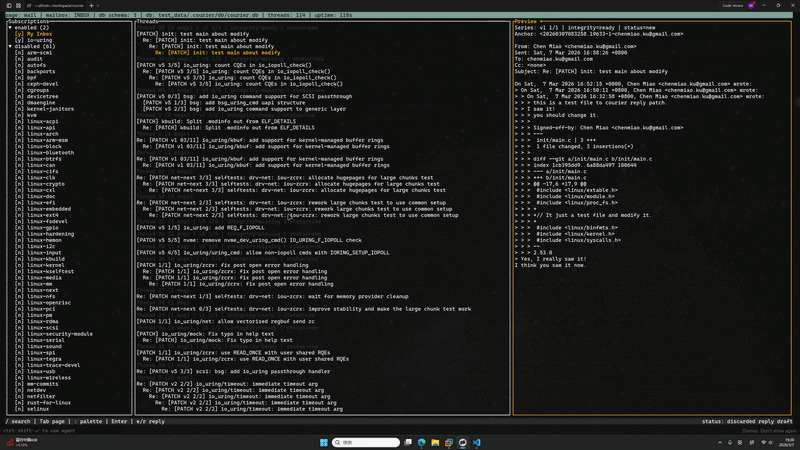
\includegraphics[width=\linewidth,height=0.6\textheight,keepaspectratio]{criew-thread-demo.png}
  \end{center}
  \vspace{0.05em}
  \begin{beamercolorbox}[wd=\linewidth,sep=0.55em,rounded=true]{block body example}
    \scriptsize
    \textbf{读图方式：}左侧是 mailbox / 订阅，中间是 thread 树，右侧是当前邮件预览；这让 patch、reply 和上下文重新回到同一屏里。
  \end{beamercolorbox}
\end{frame}

\begin{frame}
  \sectiontitle{它替你省掉哪些机械劳动}
  \small
  \begin{columns}[T,totalwidth=\textwidth]
    \begin{column}{0.32\textwidth}
      \statcard{block body alerted}{统一入口}{
        \texttt{criew doctor / sync / tui} 把入口压缩成几条命令。
      }
      \vspace{0.55em}
      \statcard{block body}{双源同步}{
        既能跟 lore 订阅，也能接 IMAP INBOX。
      }
    \end{column}
    \begin{column}{0.32\textwidth}
      \statcard{block body example}{线程建模}{
        按 Message-ID / References 重建讨论上下文。
      }
      \vspace{0.55em}
      \statcard{block body}{Patch 语义}{
        识别 [PATCH vN M/N]，自动聚合成 series。
      }
    \end{column}
    \begin{column}{0.32\textwidth}
      \statcard{block body}{b4 集成}{
        \texttt{b4 am} / \texttt{shazam} 的 apply 结果可以被追踪。
      }
      \vspace{0.55em}
      \statcard{block body alerted}{回信面板}{
        预填 Re:、To/Cc、引用正文，并先看发送预览。
      }
    \end{column}
  \end{columns}
  \vspace{0.6em}
  \begin{beamercolorbox}[wd=\linewidth,sep=0.7em,rounded=true]{block body example}
    把机械动作变成默认动作，才是降低上手门槛的关键。
  \end{beamercolorbox}
\end{frame}

\begin{frame}
  \sectiontitle{对比传统做法，CRIEW 改善了什么}
  \begin{columns}[T,totalwidth=\textwidth]
    \begin{column}{0.48\textwidth}
      \begin{alertblock}{传统链路}
        \begin{itemize}
          \item 浏览器看 lore，终端里单独 apply
          \item 邮件客户端与代码现场天然脱节
          \item 回信头与抄送名单靠手工维护
          \item thread 状态、patch 状态分散在多个工具里
        \end{itemize}
      \end{alertblock}
    \end{column}
    \begin{column}{0.48\textwidth}
      \begin{exampleblock}{CRIEW 链路}
        \begin{itemize}
          \item 订阅、thread、正文、tree 视图在同一 TUI
          \item patch apply 与邮件上下文尽量同屏
          \item reply 头与引用结构自动构造
          \item 更适合刚上手邮件协作的新同学
        \end{itemize}
      \end{exampleblock}
    \end{column}
  \end{columns}
  \vspace{0.5em}
  \begin{beamercolorbox}[wd=\linewidth,sep=0.8em,rounded=true]{block body}
    \textbf{总结：}它改善的是流程摩擦与上下文切换成本，而不是试图改写 kernel 社区规则。
  \end{beamercolorbox}
\end{frame}

\begin{frame}
  \sectiontitle{CRIEW 现在到了什么阶段}
  \scriptsize
  \begin{columns}[T,totalwidth=\textwidth]
    \begin{column}{0.48\textwidth}
      \begin{exampleblock}{已经具备}
        \begin{itemize}
          \item 当前公开版本是 \texttt{v0.0.2}。
          \item \texttt{doctor / sync / tui} 这条主链路已经可以演示和上手。
          \item 已经把 lore / IMAP 同步、thread 阅读、patch apply、reply 预览串成一套终端流程。
          \item patch 入口以 \texttt{b4} 为中心，回信路径可走 \texttt{git send-email}。
        \end{itemize}
      \end{exampleblock}
    \end{column}
    \begin{column}{0.48\textwidth}
      \begin{alertblock}{当前边界}
        \begin{itemize}
          \item 它面向 terminal-first 用户，不会变成网页式 PR 平台。
          \item 真实 IMAP、apply、发送链路仍需要本地环境和账号配置。
          \item 它替你省工具摩擦，但不替你做 maintainer 选择、测试和工程判断。
          \item 现在最适合愿意给真实 workflow 反馈的早期用户和贡献者。
        \end{itemize}
      \end{alertblock}
    \end{column}
  \end{columns}
  \vspace{0.25em}
  \begin{beamercolorbox}[wd=\linewidth,sep=0.55em,rounded=true]{block title}
    \textbf{交流会价值：}现在正是适合社区交流的阶段，核心链路已经能看见，但产品形态还在和真实使用场景一起打磨。
  \end{beamercolorbox}
\end{frame}

\begin{frame}
  \sectiontitle{CRIEW 让流程更顺，但不替代内核社区基本功}
  \small
  \begin{beamercolorbox}[wd=\linewidth,sep=0.8em,rounded=true]{block body}
    \textbf{工具负责把链路接起来；工程判断、测试质量和沟通质量仍然来自开发者本人。}
  \end{beamercolorbox}
  \vspace{0.8em}
  \begin{columns}[T,totalwidth=\textwidth]
    \begin{column}{0.48\textwidth}
      \statcard{block body alerted}{仍然要做的事}{
        选对 maintainer 和 mailing list；跑构建、测试和 \texttt{scripts/checkpatch.pl}。
      }
      \vspace{0.6em}
      \statcard{block body}{写作要求}{
        写清 commit message、cover letter 和 changelog。
      }
    \end{column}
    \begin{column}{0.48\textwidth}
      \statcard{block body example}{交流要求}{
        正确回复 review，并按节奏做 v2 / v3 reroll。
      }
      \vspace{0.6em}
      \statcard{block body}{CRIEW 的价值}{
        让新人把注意力更早放在 patch 质量与交流内容上，而不是被工具碎片卡住。
      }
    \end{column}
  \end{columns}
\end{frame}

\begin{frame}[fragile]
  \sectiontitle{会后自己上手的最短路径}
  \small
  \begin{columns}[T,totalwidth=\textwidth]
    \begin{column}{0.45\textwidth}
      \begin{beamercolorbox}[wd=\linewidth,sep=1em,rounded=true]{block body}
{\ttfamily
cargo install criew\\
criew doctor\\
criew sync --mailbox io-uring\\
criew tui
}
      \end{beamercolorbox}
      \vspace{0.5em}
      \begin{beamercolorbox}[wd=\linewidth,sep=0.7em,rounded=true]{block body example}
        第一轮建议只读公开列表，不必一上来就把真实发信链路全部接上。
      \end{beamercolorbox}
    \end{column}
    \begin{column}{0.51\textwidth}
      \begin{enumerate}
        \item 先同步一个公开列表，建立对 thread 的直觉。
        \item 在 TUI 里顺着 series 阅读 cover letter、patch、回复。
        \item 需要验证时，再把 series apply 到本地 kernel tree。
        \item 熟悉 reply 结构之后，再尝试写 review。
        \item 最后才接入 IMAP 与真实发送，把风险前移到阅读阶段。
      \end{enumerate}
    \end{column}
  \end{columns}
  \vspace{0.5em}
  \begin{beamercolorbox}[wd=\linewidth,sep=0.7em,rounded=true]{block title}
    \textbf{建议顺序：}先练阅读和 apply，再练发信。
  \end{beamercolorbox}
\end{frame}

\begin{frame}
  \sectiontitle{会后怎么试，怎么参与}
  \small
  \begin{columns}[T,totalwidth=\textwidth]
    \begin{column}{0.48\textwidth}
      \begin{exampleblock}{最快的会后动作}
        \begin{itemize}
          \item 从仓库 README 和 wiki 开始，把 \texttt{doctor / sync / tui} 这条链路跑通。
          \item 先拿一个公开列表做阅读和 thread 导航练习。
          \item 如果现场演示触发了兴趣，优先复现你自己关心的真实 thread。
        \end{itemize}
      \end{exampleblock}
    \end{column}
    \begin{column}{0.48\textwidth}
      \begin{alertblock}{最有价值的反馈}
        \begin{itemize}
          \item 带具体 mailing list thread、具体卡点和具体命令环境来反馈。
          \item 对 sync、apply、reply 三条链路的失败样本尤其有价值。
          \item 除了代码，也欢迎文档、交互、术语和新人上手路径方面的建议。
        \end{itemize}
      \end{alertblock}
    \end{column}
  \end{columns}
  \vspace{0.5em}
  \begin{beamercolorbox}[wd=\linewidth,sep=0.75em,rounded=true]{block body}
    \textbf{入口：}\href{https://github.com/ChenMiaoi/CRIEW}{CRIEW GitHub repository} \quad
    \href{https://github.com/ChenMiaoi/CRIEW/wiki}{CRIEW wiki}
  \end{beamercolorbox}
\end{frame}

\begin{frame}
  \sectiontitle{参考资料}
  \footnotesize
  \begin{itemize}
    \item \href{https://github.com/ChenMiaoi/CRIEW}{CRIEW README}
    \item \href{https://docs.kernel.org/process/}{Linux kernel process overview}
    \item \href{https://docs.kernel.org/process/submitting-patches.html}{Submitting patches}
    \item \href{https://docs.kernel.org/process/submit-checklist.html}{Patch submission checklist}
    \item \href{https://b4.docs.kernel.org/en/latest/contributor/overview.html}{b4 contributor overview}
    \item \href{https://b4.docs.kernel.org/en/latest/maintainer/am-shazam.html}{b4 am / shazam}
    \item \href{https://git-scm.com/docs/git-send-email}{git send-email}
  \end{itemize}
  \vspace{0.7em}
  \begin{beamercolorbox}[wd=\linewidth,sep=0.8em,rounded=true]{block body example}
    这份 Beamer 稿现在更适合 30 到 60 分钟社区交流会；建议现场穿插 live demo，并预留问答时间。
  \end{beamercolorbox}
\end{frame}

\end{document}
